\documentclass[10pt, a5paper]{article}
\usepackage{pdfpages}
\usepackage{parallel}
\usepackage[T2A]{fontenc}
\usepackage{ucs}
\usepackage[utf8x]{inputenc}
\usepackage[polish,english,russian]{babel}
\usepackage{hyperref}
\usepackage{rotating}
\usepackage[inner=2cm,top=1.8cm,outer=2cm,bottom=2.3cm,nohead]{geometry}
\usepackage{listings}
\usepackage{graphicx}
\usepackage{wrapfig}
\usepackage{longtable}
\usepackage{indentfirst}
\usepackage{array}
\newcolumntype{P}[1]{>{\raggedright\arraybackslash}p{#1}}
\frenchspacing
\usepackage{fixltx2e} %text sub- and superscripts
\usepackage{icomma} % коскі ў матэматычным рэжыме
\PreloadUnicodePage{4}

\newcommand{\longpage}{\enlargethispage{\baselineskip}}
\newcommand{\shortpage}{\enlargethispage{-\baselineskip}}

\def\switchlang#1{\expandafter\csname switchlang#1\endcsname}
\def\switchlangbe{
\let\saverefname=\refname%
\def\refname{Літаратура}%
\def\figurename{Іл.}%
}
\def\switchlangen{
\let\saverefname=\refname%
\def\refname{References}%
\def\figurename{Fig.}%
}
\def\switchlangru{
\let\saverefname=\refname%
\let\savefigurename=\figurename%
\def\refname{Литература}%
\def\figurename{Рис.}%
}

\hyphenation{admi-ni-stra-tive}
\hyphenation{ex-pe-ri-ence}
\hyphenation{fle-xi-bi-li-ty}
\hyphenation{Py-thon}
\hyphenation{ma-the-ma-ti-cal}
\hyphenation{re-ported}
\hyphenation{imp-le-menta-tions}
\hyphenation{pro-vides}
\hyphenation{en-gi-neering}
\hyphenation{com-pa-ti-bi-li-ty}
\hyphenation{im-pos-sible}
\hyphenation{desk-top}
\hyphenation{elec-tro-nic}
\hyphenation{com-pa-ny}
\hyphenation{de-ve-lop-ment}
\hyphenation{de-ve-loping}
\hyphenation{de-ve-lop}
\hyphenation{da-ta-ba-se}
\hyphenation{plat-forms}
\hyphenation{or-ga-ni-za-tion}
\hyphenation{pro-gramming}
\hyphenation{in-stru-ments}
\hyphenation{Li-nux}
\hyphenation{sour-ce}
\hyphenation{en-vi-ron-ment}
\hyphenation{Te-le-pathy}
\hyphenation{Li-nux-ov-ka}
\hyphenation{Open-BSD}
\hyphenation{Free-BSD}
\hyphenation{men-ti-on-ed}
\hyphenation{app-li-ca-tion}

\def\progref!#1!{\texttt{#1}}
\renewcommand{\arraystretch}{2} %Іначай формулы ў матрыцы зліпаюцца з лініямі
\usepackage{array}

\def\interview #1 (#2), #3, #4, #5\par{

\section[#1, #3, #4]{#1 -- #3, #4}
\def\qname{LVEE}
\def\aname{#1}
\def\q ##1\par{{\noindent \bf \qname: ##1 }\par}
\def\a{{\noindent \bf \aname: } \def\qname{L}\def\aname{#2}}
}

\def\interview* #1 (#2), #3, #4, #5\par{

\section*{#1\\{\small\rm #3, #4. #5}}

\def\qname{LVEE}
\def\aname{#1}
\def\q ##1\par{{\noindent \bf \qname: ##1 }\par}
\def\a{{\noindent \bf \aname: } \def\qname{L}\def\aname{#2}}
}

\begin{document}
\title{Низкоуровневый взгляд на динамические ELF-библиотеки\footnote{\url{punkofnewsociety@gmail.com}, \url{https://lvee.org/en/abstracts/280}, материал распространяется под лицензией Attribution 4.0 International (CC BY 4.0)}}
\author{Uladzislau Zhauniarovich, Minsk, Belarus}
\maketitle
\begin{abstract}
Complex applications work with dynamically linked libraries. Statically linked applications would be very large and have lack of flexibility as with dynamic libraries, because one library can be used by several applications at once.
The purpose of this report is precisely to focus on all low-level features of working with these libraries, including such mechanisms like 
ELF sections, symbol relocations, GOT(global offset table), PLT(procedure linkage table).
\end{abstract}
\section*{Введение}

На примере языка программирования Си можно выделить три основных этапа с момента написания программного кода до работы получившейся программы в операционной системе. 
Это препроцессинг, компиляция, компоновка/линковка. Остановимся на последнем этапе. К этому времени инструкции в процессе компиляции в  основном сгенерированы.  Компоновщик~--- это программа, которая выбирает адреса для всех символов(глобальные переменные и функции, либо вспомогательные debug-символы). Без компоновщика мы бы не могли делать раздельную компиляцию. Много обьектных файлов не нужно перекомпилировать с самого начала, если в них нету изменений и пересборка идет только в файлах с изменениями(прим. open office, linux kernel).

ELF~--- Executable and Linkable Format. Эти файлы можно разделить на три категории:

\begin{itemize}
  \item Relocatable files~--- .o (то что получается после компиляции) является элементом static libraries (.a), т.е. может включать 1 или больше.
  \item Executable~--- программы после этапа линковки, готовые к запуску.
  \item Shared~--- .so dynamic libraries, они должны быть скомпонованы с запускаемым файлом в run-time.
\end{itemize}

Релокация~--- это процесс подстановки символу его адреса. 

Static linker превращает первую категорию во вторую или третью.

Dynamic linker подготавливает третью к выполнению.

\section*{Инструменты для анализа бинарных файлов}

Список таких инструментов включает:

\begin{itemize}
  \item readelf~--- получение специфичной для формата ELF информации.
  \item objdump~--- дизассемблер, позволяет исследовать обьектные файлы разных форматов.
  \item nm~--- просмотр символов, которые есть в ELF-файле.
\end{itemize}

В набор GNU Binutils также входят elfedit, elfdump и др., но в данном контексте они не понадобятся.

\section*{Структура ELF, содержимое секций}

ELF-файл содержит 3 заголовка~--- File Header, Program Header, и Section Header.
Заголовок ELF-файла содержит magic number 7f 45 4c 46 ( 7f + ascii коды букв ELF) и указатели на Program Header и Section Header.

Program Header формируется при помощи компоновщика и содержит 
информацию о сегментах. Сегменты~--- это регионы памяти, которые содержат некоторое количество секций.

Section Header содержит информацию про секции .text .data .bss .rodata и множество служебных секций .symtab .line .strtab .debug .got .got.plt. Он необходим для линковки.
\newpage
\begin{center}
\begin{figure}[h!]
  \centering
  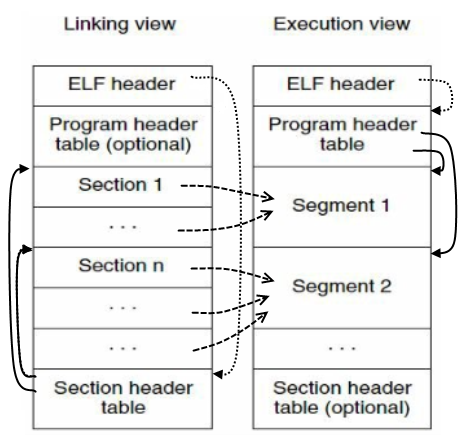
\includegraphics[width=7cm]{12_2018_Zhauniarovich1.png}
  %\caption{Блок-схема примерной системы распознавания РОГ}
  \label{Zhauniarovich1}
\end{figure}
\end{center} 

\section*{Релокации, GOT, PLT}

Когда линкер создает разделяемую библиотеку, он заранее не знает, в каком месте в памяти она будет загружена. Из-за этого делать ссылки на данные и код внутри библиотеки проблематично: непонятно, как создавать ссылку, чтобы она указывала в правильное место после того, как библиотека будет загружена.

В Linux и в ELF существует два главных способа решить эту проблему:

\begin{itemize}
  \item релокация во время загрузки (load-time relocation);
  \item код, не зависящий от адреса (position-independent code, PIC).
\end{itemize}

Релокация во время загрузки~--- это очень простой и прямолинейный метод. И он работает. Но PIC гораздо более популярен на данный момент и является рекомендуемым способом создания разделяемых библиотек.

У load-time relocation есть проблемы: она занимает время, и секция text (содержащая машинный код) уже не подходит для разделения между процессами.

Поэтому существует такая модель, как Global Offset Table. 
GOT~--- это просто таблица с адресами, которая находится в секции data.

Предположим, что какая-то инструкция в секции code хочет обратиться к переменной. Вместо того, чтобы обратится к ней через абсолютный адрес (который потребует релокации), она обращается к записи в GOT. Поскольку GOT имеет строго определённое место в секции data, и линкер знает о нём, это обращение тоже является относительным. А запись в GOT уже содержит абсолютный адрес переменной:

\begin{center}
\begin{figure}[h!]
  \centering
  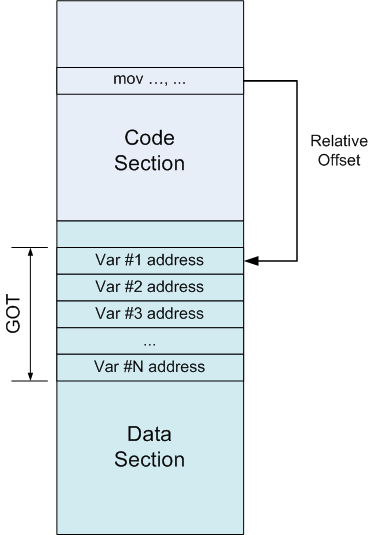
\includegraphics[width=5cm]{12_2018_Zhauniarovich2.png}
  %\caption{Блок-схема примерной системы распознавания РОГ}
  \label{Zhauniarovich2}
\end{figure}
\end{center} 

Однако суть разделяемых библиотек на сегодняшний день в том, что в них может содержаться 10 000 различных функций, но использовать оттуда мы, например, будем лишь № 1 или № 4. Чтобы каждый раз подгружать абсолютно все функции в GOT, мы используем процедуру <<ленивого связывания>>, т.е. связывание функции из библиотеки с программой происходит при непосредственном вызове её. Помогает в этом механизм Procedure Linkage Table (PLT).

PLT~--- это часть секции text в бинарнике, состоящая из набора элементов (один элемент на одну внешнюю функцию, которую вызывает библиотека). Каждый элемент в PLT~--- это небольшой кусок выполняемого машинного кода. Вместо вызова функции напрямую вызывается кусок кода из PLT, который уже сам вызывает функцию. Такой подход часто называют <<трамплином>>. Каждый элемент из PLT имеет собственный элемент в GOT, который содержит реальное смещение для функции (конечно после того как загрузчик определит её).

\begin{center}
\begin{figure}[h!]
  \centering
  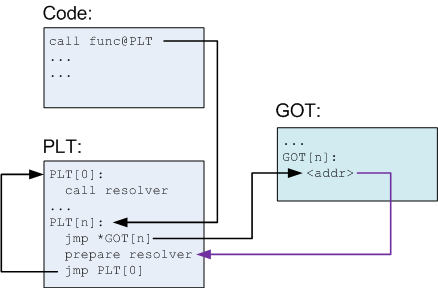
\includegraphics[width=5cm]{12_2018_Zhauniarovich3.png}
  %\caption{Блок-схема примерной системы распознавания РОГ}
  \label{Zhauniarovich3}
\end{figure}
\end{center} 

В коде вызывается функция func. Компилятор переводит этот вызов в вызов func@plt, который является одним из элементов PLT. После этого идет обращение в GOT, и с учетом того что функция вызывалась в первый раз~--- управление передаётся обратно PLT, где т. н. resolver устанавливает связь между названием функции и её кодом из библиотеки. После такого первого связывания схема будет выглядеть немного по-другому:

\begin{center}
\begin{figure}[h!]
  \centering
  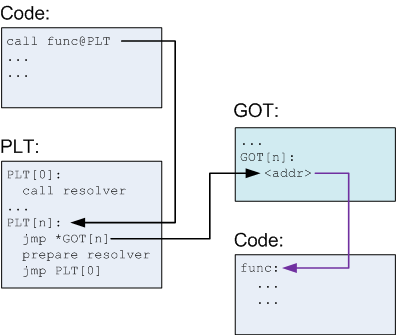
\includegraphics[width=5cm]{12_2018_Zhauniarovich4.png}
  %\caption{Блок-схема примерной системы распознавания РОГ}
  \label{Zhauniarovich4}
\end{figure}
\end{center} 

Библиотека при этом абсолютно не зависит от адреса, по которому она будет загружена: ведь единственное место, где используется абсолютный адрес~--- это GOT, а она находится в секции data и будет релоцирована загрузчиком во время загрузки. Даже PLT не зависит от адреса загрузки, так что она может находиться в секции text, доступной только для чтения.

\section*{Эксперимент с перенаправлением обращений к функциям из библиотек}

Наглядно продемонстрировать описанные процессы можно в ходе эксперимента с использованием предварительно написанной демонстрационной программы, функциональность которой должна включать:

\begin{itemize}
  \item создание паттерна <<Proxy>> для вызова функций (которые, в свою очередь, используют системные функции) из заранее откопилированных (пользовательских) библиотек без их прямого изменения;
  \item перенаправление их вызовов в свой интерфейс, для дальнейшего вызова тех самых системных функций из пользовательских библиотек.
\end{itemize}

\end{document}
